\documentclass[handout,nooutcomes]{ximera}
%% handout
%% space
%% newpage
%% numbers
%% nooutcomes

%I added the commands here so that I would't have to keep looking them up
%\newcommand{\RR}{\mathbb R}
%\renewcommand{\d}{\,d}
%\newcommand{\dd}[2][]{\frac{d #1}{d #2}}
%\renewcommand{\l}{\ell}
%\newcommand{\ddx}{\frac{d}{dx}}
%\everymath{\displaystyle}
%\newcommand{\dfn}{\textbf}
%\newcommand{\eval}[1]{\bigg[ #1 \bigg]}

%\begin{image}
%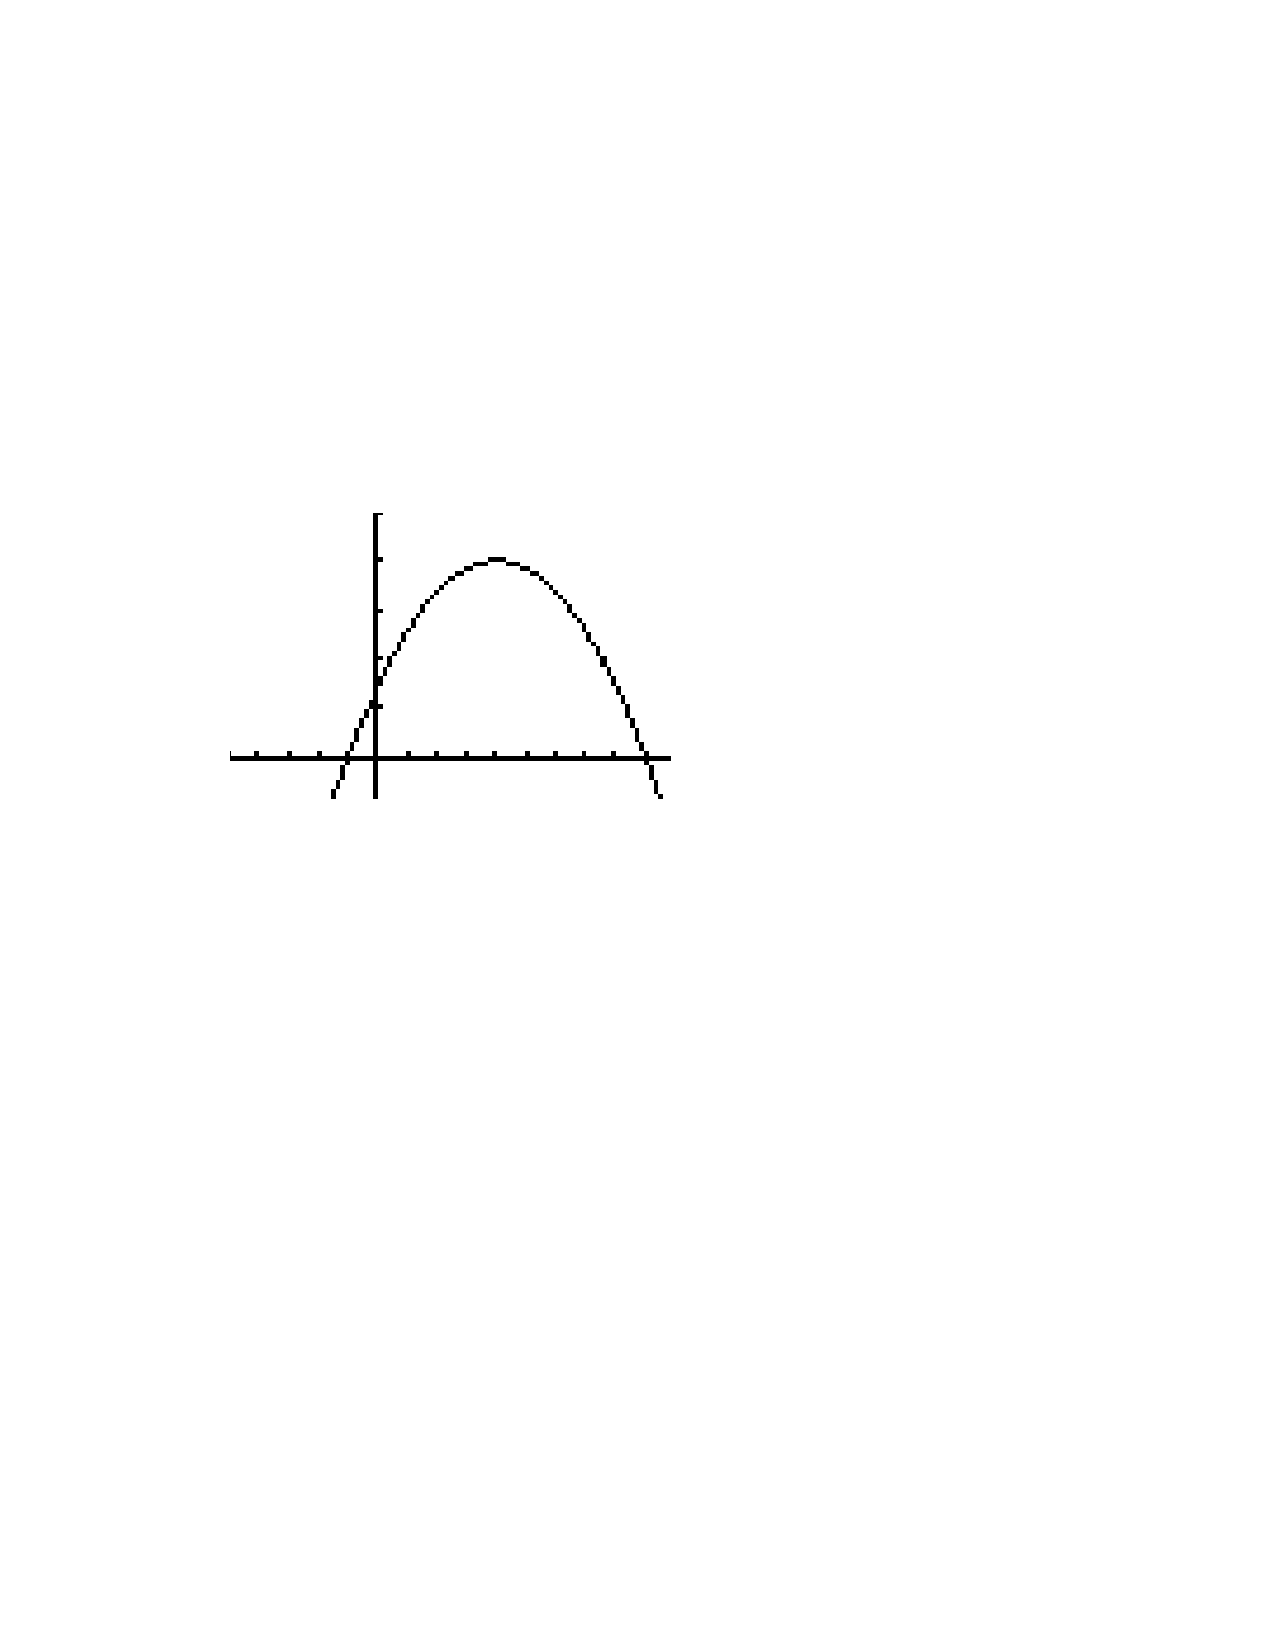
\includegraphics[trim= 170 420 250 180]{Figure1.pdf}
%\end{image}


\newcommand{\RR}{\mathbb R}
\renewcommand{\d}{\,d}
\newcommand{\dd}[2][]{\frac{d #1}{d #2}}
\renewcommand{\l}{\ell}
\newcommand{\ddx}{\frac{d}{dx}}
\newcommand{\dfn}{\textbf}
\newcommand{\eval}[1]{\bigg[ #1 \bigg]}

\usepackage{multicol}

\renewenvironment{freeResponse}{
\ifhandout\setbox0\vbox\bgroup\else
\begin{trivlist}\item[\hskip \labelsep\bfseries Solution:\hspace{2ex}]
\fi}
{\ifhandout\egroup\else
\end{trivlist}
\fi} %% we can turn off input when making a master document

\title{Recitation \#25 - 5.3 Fundamental Theorem of Calculus Part II}  

\begin{document}
\begin{abstract}		\end{abstract}
\maketitle

\section*{Warm up:} 
How do the functions $f(x) = \left( e^x \right)^2$ and $g(x) = e^{x^2}$ differ, and how does that effect the computations of the integrals:
$$ \int_0^1 \left(e^x \right)^2 \d x	\qquad	\text{and}	\qquad	\int_0^1 e^{x^2} \d x $$
		\begin{freeResponse}
		$f(x) = \left( e^x \right)^2 = e^x \cdot e^x = e^{x+x} = e^{2x}$.  
		So $f(x) \neq g(x)$ since $2x \neq x^2$.  
		Then,
			\begin{align*}
			\int_0^1 f(x) \d x &= \int_0^1 \left(e^x \right)^2 \d x  \\
			&= \int_0^1 e^{2x} \d x  \\
			&= \eval{\frac{1}{2} e^{2x}}_0^1  \\
			&= \frac{1}{2} \left( e^2 - e^0 \right)  \\
			&= \frac{1}{2} \left( e^2 - 1 \right).  
			\end{align*}
			
		We do not have the tools to prove it in this class, but $g(x) = e^{x^2}$ does not have a ``closed form" antiderivative.  
		Therefore, we do not have a nice way to compute $\int_0^1 e^{x^2} \d x$ using the Fundamental Theorem of Calculus (Part II).
		\end{freeResponse}	
		
		
		

	
	
	
	
	

\section*{Group work:}



%problem 1
\begin{problem}
Compute the following definite integrals:
	\begin{enumerate}
	
	%part a
	\item  $\int_0^3 \frac{6}{9 + x^2} \d x $
		\begin{freeResponse}
			\begin{align*}
			\int_0^3 \frac{6}{9 + x^2} \d x &= 6 \int_0^3 \frac{1}{9 + x^2} \d x  \\
			&= 6 \int_0^3 \frac{1}{(3)^2 + x^2} \d x  \\
			&= \eval{6 \cdot \frac{1}{3} \arctan \left( \frac{x}{3} \right)}_0^3  \\
			&= 2 \eval{ \arctan \left( \frac{x}{3} \right)}_0^3  \\
			&= 2 \left( \frac{\pi}{4} - 0 \right) = \frac{\pi}{2}
			\end{align*}
		\end{freeResponse}
		
		
		
	%part b
	\item  $\int_0^{\frac{\pi}{4}} \sec^2 (x) \d x$
		\begin{freeResponse}
		$\int_0^{\frac{\pi}{4}} \sec^2 (x) \d x = \eval{\tan(x)}_0^{\frac{\pi}{4}} = 1 - 0 = 1$
		\end{freeResponse}
		
		
		
	%part c
	\item  $\int_1^4 \frac{x^3 + 7x + 5}{x} \d x$
		\begin{freeResponse}
			\begin{align*}
			\int_1^4 \frac{x^3 + 7x + 5}{x} \d x &= \int_1^4 \left( \frac{x^3}{x} + \frac{7x}{x} + \frac{5}{x} \right) \d x  \\
			&= \int_1^4 ( x^2 + 7 + 5x^{-1} ) \d x  \\
			&= \eval{\frac{1}{3} x^3 + 7x + 5\ln |x| }_1^4  \\
			&= \left( \frac{64}{3} + 28 + 5\ln(4) \right) - \left( \frac{1}{3} + 7 + 5 \ln(1) \right)  \\
			&= 21 + 21 + 5\ln(4) = 42 + 5\ln(4)
			\end{align*}
		\end{freeResponse}
		
		
		
	%part d
	\item  $\int_{- \frac{\pi}{2}}^0 \cos^2 (x) \d x$
		\begin{freeResponse}
		The key to solve this integral is to recall that
		$$ \cos^2 (x) = \frac{1}{2} \left( 1 + \cos(2x) \right) .$$
		Once you have that, the problem is straightforward:
			\begin{align*}
			\int_{- \frac{\pi}{2}}^0 \cos^2 (x) \d x &= \frac{1}{2} \int_{- \frac{\pi}{2}}^0 \left( 1 + \cos(2x) \right) \d x  \\
			&= \frac{1}{2} \eval{ x + \frac{1}{2} \sin(2x)  }_{- \frac{\pi}{2}}^0  \\
			&= \frac{1}{2} \left[ (0 + 0) - \left(- \frac{\pi}{2} + 0 \right) \right]  \\
			&= \frac{\pi}{4}
			\end{align*}
		\end{freeResponse}
		
		
		
	\end{enumerate}
		
		
\end{problem}



After completing problem 1, review for Midterm 3.


















	
	
	
	
	
	
	
	
	

	










								
				
				
	














\end{document} 


















